\documentclass[12pt]{article}

\usepackage[a4paper,margin=2.5cm]{geometry}
\usepackage{graphicx}
\usepackage{url}
\usepackage[utf8]{inputenc}
\usepackage[T1]{fontenc}
\usepackage[brazil]{babel}

\usepackage{amsmath,amssymb,amsfonts}
\usepackage{booktabs}
\usepackage{multirow}
\usepackage{array}
\usepackage{enumitem}
\usepackage[hidelinks]{hyperref}
\graphicspath{{../resultados/}}
\newenvironment{resumo}{%
  \renewcommand{\abstractname}{Resumo}\begin{abstract}%
}{\end{abstract}}

% Permite que URLs longas quebrem de linha (sem perder o link)
\Urlmuskip=0mu plus 1mu\relax
\makeatletter
\g@addto@macro\UrlBreaks{\do\/\do\-\do\.\do\_\do\?\do\&\do\=\do\#\do\:}
\makeatother

\sloppy

\title{Predição Espaço-Temporal de Acidentes de Trânsito em Rodovias
Federais de Minas Gerais com Graph Neural Networks e Representação
Estrutural da Malha Viária}

\author{
Giovanni Willik Del Piccolo,
João Victor De Pascale Souza,
Lion Chen\\
Universidade de São Paulo (USP)\\
São Paulo -- SP -- Brasil\\
\texttt{\{15455979,15463888,15470010\}}
}
\date{Versão final organizada -- novembro de 2026}

\begin{document}

\maketitle

% ============================================================
\begin{abstract}
Traffic accidents on Minas Gerais (MG, Brazil) federal highways constitute a significant
public health problem. This work proposes the use of Graph Neural
Networks for spatiotemporal accident prediction
on federal highways, representing the road network as a georeferenced
graph based on open data from the Brazilian Federal Highway Police
(PRF). Random Forest, XGBoost, MLP, GraphSAGE and GATv2 were trained
and evaluated using five random seeds and temporal splits. The
experiment comprised 25 full-model runs and 30 graph-model ablations.
XGBoost achieved the highest mean average precision in 2025 (0.1675)
and in the partial 2026 test (0.1723). The graph-based models did not
outperform the tabular references under this protocol. Dataset
reconstruction and inference replay reproduced the recorded metrics
without retraining in the same installed runtime. These findings are
conditional on assumed temporal data coverage and a limited training
budget.
\end{abstract}

\begin{resumo}
Acidentes de trânsito em rodovias federais de Minas Gerais (MG, Brasil) constituem um
importante problema de saúde pública. Este trabalho propõe o uso de
Graph Neural Networks para a predição
espaço-temporal de acidentes em rodovias federais, representando a
malha viária como um grafo georreferenciado a partir de dados abertos
da Polícia Rodoviária Federal (PRF). Random Forest, XGBoost, MLP,
GraphSAGE e GATv2 foram implementados, treinados e avaliados com cinco
sementes e divisão temporal, totalizando 25 treinamentos completos e
30 ablações das GNNs. XGBoost obteve a maior precisão média (AP) em
2025 (0,1675) e no teste parcial de 2026 (0,1723). Os modelos em grafo
não superaram as referências tabulares neste protocolo. A
reconstrução dos dados e a repetição das inferências reproduziram as
métricas registradas, sem novo treinamento e no mesmo ambiente
instalado. Os resultados reportados são
condicionados à hipótese de cobertura temporal dos dados e ao
orçamento limitado de treinamento.
\end{resumo}

% ============================================================
\section{Introdução}

O Brasil apresenta um importante problema de segurança viária, com
impactos significativos sobre a saúde pública e a sociedade
\cite{who2023}. Nas rodovias federais, a Polícia Rodoviária Federal
(PRF) contabilizou 72.483 sinistros em 2025, resultando em 6.044 mortes
\cite{prf2026}. Esses números reforçam a importância de compreender os
fatores associados à ocorrência de acidentes e de desenvolver métodos
capazes de identificar padrões e antecipar situações de maior risco.

Nesse contexto, Araújo \cite{araujo2022} investigou padrões associados
aos acidentes em rodovias federais brasileiras utilizando dados da
Polícia Rodoviária Federal e algoritmos de regras de associação, como
Apriori, Eclat, FP-Growth e FP-Max. O estudo analisou relações entre
características dos acidentes, dos veículos, das vias e do ambiente,
contribuindo para a identificação de combinações de fatores
frequentemente associadas aos acidentes.

A partir dessa abordagem, este trabalho propõe uma extensão da análise
por meio de técnicas de aprendizado profundo em grafos. Em vez de
considerar os registros de acidentes apenas como observações
independentes, a proposta representa a malha rodoviária como um grafo
georreferenciado, no qual os segmentos da rodovia são representados
como nós e suas relações de conectividade como arestas. Essa
representação permite incorporar explicitamente a dimensão espacial
dos acidentes e investigar como informações de segmentos próximos
podem contribuir para a predição de ocorrências.

O uso de Graph Neural Networks para a análise e predição de acidentes
de trânsito já foi explorado em trabalhos recentes. Zhang et al.
\cite{zhang2026} propuseram uma abordagem baseada em representações
em grafos para a predição de acidentes, combinando informações da rede
viária com características temporais, ambientais e imagens de
satélite. O estudo utilizou dados de acidentes de seis estados dos
Estados Unidos e demonstrou o potencial das representações em grafos
para essa tarefa, alcançando desempenho superior quando diferentes
fontes de informação foram combinadas. Entretanto, essa abordagem foi
desenvolvida para o contexto norte-americano, não tendo sido aplicada
à realidade das rodovias federais brasileiras.

Este trabalho busca explorar essa abordagem no contexto brasileiro,
utilizando os dados abertos da Polícia Rodoviária Federal e a
representação geográfica da malha de rodovias federais como um grafo.
Foram avaliadas Graph Neural Networks, com foco nos modelos GraphSAGE
e GATv2, para a predição espaço-temporal de acidentes. Modelos
tabulares, como XGBoost, Random Forest e MLP, também foram utilizados
como referência, permitindo comparar uma abordagem baseada nas
características dos segmentos com outra que considera
explicitamente as relações estruturais da malha rodoviária. Este
relatório consolida os resultados existentes dos cinco modelos, as
ablações e a reprodução registrada em setembro de 2026. A organização
dos arquivos e a atualização deste texto não envolveram novos
treinamentos, alterações de código nem seleção pelos resultados dos
testes. Dessa forma, o trabalho
busca complementar a análise realizada por Araújo \cite{araujo2022},
investigando o potencial da representação em grafos para a análise e
predição de acidentes de trânsito no Brasil, a partir dos resultados
preliminares já obtidos com os modelos tabulares.

% ============================================================


\section{Trabalhos Relacionados}
Esta seção discute cinco trabalhos diretamente relacionados à proposta,
analisando em profundidade seus objetivos, métodos, resultados e
limitações. Os dois primeiros (Araújo \cite{araujo2022} e Zhang et
al. \cite{zhang2026}) constituem os trabalhos-base desta pesquisa: o
primeiro define o domínio de aplicação (acidentes em rodovias federais
brasileiras) e o segundo, a estratégia metodológica (representação em
grafo e Graph Neural Networks). Os três seguintes (Nippani et al.
\cite{nippani2023}, Gao et al. \cite{zhuang2024} e Amorim et al.
\cite{amorim2023}) fundamentam decisões metodológicas específicas e
contextualizam a aplicação no cenário brasileiro. A subseção final
sintetiza como cada trabalho se relaciona com a presente proposta.

\subsection{Araújo (2022): regras de associação em rodovias federais}

O trabalho de Araújo \cite{araujo2022}, desenvolvido na UFMG, é o ponto
de partida desta pesquisa. O autor aplicou algoritmos de regras de
associação (Apriori, Eclat, FP-Growth e FP-Max) sobre dados
abertos da PRF referentes ao período de janeiro de 2017 a fevereiro de
2020, com o objetivo de identificar relações entre as causas dos
acidentes e características dos veículos, das estradas, dos usuários e
do ambiente. A base de acidentes foi enriquecida com atributos dos
veículos obtidos do RENAVAM, como potência, cilindrada, combustível e
número de eixos, e submetida a etapas de limpeza e transformação antes
da geração das regras.

Como resultado, o estudo constatou que Apriori, FP-Growth e Eclat
apresentam comportamento semelhante quanto às métricas de suporte e à
quantidade de características das regras, ao passo que o FP-Max produz
resultados distintos, com maior suporte para regras que envolvem mais
características. A principal contribuição é demonstrar o potencial dos
dados da PRF para revelar combinações de fatores associadas aos
acidentes. Contudo, o trabalho apresenta duas limitações centrais que
motivam a presente pesquisa: (i) é essencialmente \textit{descritivo},
identificando co-ocorrências, mas não produzindo um modelo capaz de
\textit{prever} a ocorrência de novos acidentes; e (ii) trata cada
registro isoladamente, sem considerar a dimensão espacial da rede
viária, ou seja, a possibilidade de que trechos vizinhos compartilhem
fatores de risco.

\subsection{Zhang et al. (2026): GNN multimodal para predição de acidentes}

O trabalho de Zhang et al. \cite{zhang2026}, publicado no KDD 2026, é a
principal referência metodológica desta pesquisa. Os autores propuseram
uma abordagem baseada em Graph Neural Networks para a predição de
acidentes, na qual a malha viária é representada como um grafo e cada nó
é enriquecido com múltiplas modalidades de dados: imagens de satélite de
alta resolução, estatísticas meteorológicas e tipo de via, enquanto as
arestas recebem informações de volume de tráfego. Para isso,
construíram um extenso conjunto de dados multimodal com cerca de nove
milhões de registros de acidentes distribuídos por seis estados dos
Estados Unidos.

A avaliação demonstrou que a fusão das diferentes modalidades supera os
modelos que utilizam apenas a estrutura do grafo, alcançando AUROC médio
de 90,1\%, com ganho de 3,7 pontos percentuais em relação à variante sem
as imagens de satélite. Esse resultado evidencia tanto o valor da
representação em grafo quanto o das características do entorno físico da
via. Duas características do estudo, entretanto, delimitam a lacuna
explorada neste trabalho: a abordagem foi desenvolvida e validada
exclusivamente para o contexto norte-americano, e depende de um
\textit{pipeline} de processamento de imagens de satélite de elevada
complexidade computacional, fonte de dados custosa e de difícil
reprodução no contexto brasileiro. A presente proposta herda a
estratégia de modelagem em grafo, mas a adapta às rodovias federais
brasileiras e a simplifica, dispensando modalidades de difícil obtenção.

\subsection{Nippani et al. (2023): benchmark de GNNs para segurança viária}

Nippani et al. \cite{nippani2023} estabeleceram um \textit{benchmark}
sistemático para a predição de acidentes em redes viárias por meio de
Graph Neural Networks, abordando a ausência de consenso sobre a acurácia
efetiva dos métodos existentes. Os autores modelaram a malha viária dos
Estados Unidos como um grafo, com base em conexões da rede e volume de
tráfego, e avaliaram diferentes arquiteturas na predição tanto da
contagem quanto da ocorrência de acidentes.

Entre os principais achados, modelos como o GraphSAGE preveem o número
de acidentes com erro absoluto médio relativo inferior a 22\% e a
ocorrência (classificação binária) com AUROC superior a 87\%, superando
métodos que ignoram a estrutura do grafo. Esse trabalho é particularmente
relevante para a presente pesquisa por três razões: valida
empiricamente o GraphSAGE, uma das arquiteturas aqui adotadas,
para a predição de acidentes; fornece uma referência metodológica de
avaliação por AUROC, sem comparação numérica direta entre populações
e protocolos distintos; e
confirma que a modelagem topológica agrega valor preditivo em relação a
abordagens que tratam segmentos isoladamente. Sua limitação, do ponto de
vista desta proposta, é novamente o foco no contexto norte-americano.

\subsection{Gao et al. (2024): GNN probabilística e o desafio da esparsidade}

Gao et al. \cite{zhuang2024} propuseram a STZITD-GNN
(\textit{Spatiotemporal Zero-Inflated Tweedie Graph Neural Network}),
uma GNN probabilística com quantificação de incerteza voltada à predição
de acidentes em nível de segmento viário. O trabalho parte de uma
constatação central para qualquer modelo de predição de acidentes: os
dados são dominados por valores nulos (segmentos e períodos sem
ocorrência), com raros valores altos correspondentes a eventos graves.
Essa distribuição fortemente desbalanceada e esparsa faz com que métodos
determinísticos tradicionais falhem em escalas espaço-temporais finas.

Para enfrentar esse problema, os autores empregam uma distribuição de
Tweedie \textit{zero-inflated} que modela explicitamente o excesso de
zeros, além de estimar a incerteza das predições, informação valiosa
para identificar em quais segmentos o modelo é confiável. Este trabalho
é diretamente relevante para a presente pesquisa porque o desafio da
esparsidade também estará presente na predição por trecho e janela
temporal proposta: a maioria dos pares trecho-semana não registrará
acidentes. As estratégias discutidas por Gao et al., como a ponderação
de classes e a modelagem explícita do desbalanceamento, informam o
tratamento do desbalanceamento no presente trabalho. Random Forest
usou ponderação balanceada das classes; XGBoost e as redes neurais
usaram pesos calculados somente a partir dos alvos de treinamento.

\subsection{Amorim et al. (2023): aprendizado de máquina em rodovias federais brasileiras}

Amorim et al. \cite{amorim2023} aplicaram aprendizado de máquina à
classificação de \textit{hotspots} de acidentes em rodovias federais
brasileiras, distinguindo áreas associadas a risco severo ou não severo.
Os autores compararam três algoritmos (Support Vector Machine (SVM),
Random Forest e uma rede neural do tipo \textit{multilayer perceptron}) sobre um conjunto de atributos que inclui localização espacial, dia
e horário da ocorrência, tipo e orientação da via, condições
meteorológicas e tipo de acidente. A rede neural obteve o melhor
desempenho, com acurácia de 83\%, precisão de 84\% e F1-score de 82\%.

Este trabalho é relevante para a presente pesquisa por dois motivos.
Primeiro, situa-se exatamente no mesmo domínio de aplicação (rodovias
federais brasileiras a partir de dados da PRF) confirmando a
viabilidade de modelos preditivos supervisionados sobre essa base, em
contraste com a abordagem descritiva de Araújo \cite{araujo2022}.
Segundo, os algoritmos avaliados (Random Forest e MLP, em particular)
são justamente parte do conjunto de modelos tabulares de referência
adotados neste trabalho, o que torna seus resultados um ponto de
comparação pertinente. Sua limitação, do ponto de vista desta proposta,
é não representar a rede viária como um grafo: os \textit{hotspots} são
classificados isoladamente, sem propagação de informação entre segmentos
vizinhos.

\subsection{Relação com a presente pesquisa}

Os cinco trabalhos analisados delimitam com clareza a contribuição desta
pesquisa. De um lado, os estudos no contexto brasileiro
\cite{araujo2022,amorim2023} exploram a riqueza dos dados da PRF, mas
permanecem no paradigma descritivo (regras de associação) ou em modelos
que tratam cada ocorrência isoladamente, sem representar a estrutura da
malha viária. De outro, os avanços em Graph Neural Networks para
predição de acidentes \cite{zhang2026,nippani2023,zhuang2024} demonstram
o valor da modelagem topológica e oferecem soluções para desafios como a
esparsidade, mas foram desenvolvidos e validados sobre redes viárias
norte-americanas, por vezes dependendo de fontes de dados custosas.

A Tabela~\ref{tab:comparacao} sintetiza a comparação entre os trabalhos
analisados e a presente proposta, considerando o contexto de aplicação,
os dados utilizados, a técnica empregada, a tarefa abordada, o uso de
representação em grafo e os principais resultados e limitações.

\begin{table}[!ht]
\centering
\caption{Comparação entre os trabalhos relacionados e a presente proposta.}
\label{tab:comparacao}
\footnotesize
\setlength{\tabcolsep}{2pt}
\renewcommand{\arraystretch}{1.15}
\resizebox{\textwidth}{!}{%
\begin{tabular}{>{\raggedright\arraybackslash}p{1.6cm}
                >{\raggedright\arraybackslash}p{2.4cm}
                >{\raggedright\arraybackslash}p{2.2cm}
                >{\raggedright\arraybackslash}p{2.1cm}
                >{\raggedright\arraybackslash}p{2.7cm}
                >{\centering\arraybackslash}p{1.05cm}
                >{\raggedright\arraybackslash}p{2.5cm}}
\toprule
\textbf{Trabalho} & \textbf{Contexto e dados} & \textbf{Técnica} &
\textbf{Tarefa} & \textbf{Meta (alvo de previsão)} & \textbf{Grafo} & \textbf{Resultados e limitações} \\
\midrule
Araújo \cite{araujo2022} &
Rodovias federais (Brasil); PRF 2017--2020 e RENAVAM &
Regras de associação (Apriori, Eclat, FP-Growth, FP-Max) &
Descrição de padrões entre causas e fatores &
Não aplicável --- mineração descritiva, sem alvo de previsão &
Não &
FP-Max com maior suporte para regras extensas; abordagem descritiva, sem predição \\
\midrule
Zhang et al. \cite{zhang2026} &
Seis estados (EUA); $\sim$9 milhões de acidentes, imagens de satélite, clima e tráfego &
GNN multimodal (grafo e \textit{embeddings} visuais) &
Predição de ocorrência de acidentes &
Ocorrência (sim/não) de acidente por nó da rede viária &
Sim &
AUROC médio de 90,1\% (+3,7 p.p. com imagens); depende de imagens de satélite \\
\midrule
Nippani et al. \cite{nippani2023} &
Malha viária (EUA); conexões e volume de tráfego &
\textit{Benchmark} de GNNs (p.\,ex., GraphSAGE) &
Contagem e ocorrência de acidentes &
Nº de acidentes por via (contagem) e ocorrência (sim/não) por via &
Sim &
AUROC $>$87\% e MAE relativo $<$22\%; restrito ao contexto norte-americano \\
\midrule
Gao et al. \cite{zhuang2024} &
Acidentes em nível de segmento viário &
GNN probabilística (STZITD-GNN, Tweedie \textit{zero-inflated}) &
Predição multi-passo de risco com incerteza &
Contagem/risco de acidentes por segmento, em múltiplos passos de tempo &
Sim &
Modela o excesso de zeros e quantifica a incerteza; maior complexidade do modelo \\
\midrule
Amorim et al. \cite{amorim2023} &
Rodovias federais (Brasil); dados da PRF &
SVM, Random Forest e MLP &
Classificação de \textit{hotspots} (severo / não severo) &
Classe de risco do \textit{hotspot}: severo vs. não severo &
Não &
MLP com acurácia de 83\% e F1 de 82\%; \textit{hotspots} avaliados isoladamente \\
\midrule
\textbf{Este trabalho} &
Rodovias federais de MG; PRF 2019--2026 e malha OSM (2018) &
GraphSAGE e GATv2; \textit{baselines}: XGBoost, RF e MLP &
Ocorrência de acidente por segmento e semana &
Houve $\geq$1 acidente (sim/não) por segmento $\times$ semana &
Sim &
XGBoost com maior AP nos dois testes; GNNs não superaram as referências sob cobertura assumida e orçamento limitado \\
\bottomrule
\end{tabular}
}
\end{table}

Esta proposta situa-se precisamente na interseção dessas duas frentes.
Dos trabalhos-base, herda o domínio de aplicação de Araújo
\cite{araujo2022}, que estende do descritivo para o preditivo, e a
estratégia metodológica de Zhang et al. \cite{zhang2026}, que adapta
ao contexto brasileiro e simplifica, dispensando imagens de satélite. Dos
demais, incorpora a validação do GraphSAGE para predição de acidentes
\cite{nippani2023}, o tratamento da esparsidade inerente ao problema
\cite{zhuang2024} e o uso de modelos tabulares (Random Forest, MLP) como
referência \cite{amorim2023}. Assim, aplica Graph Neural Networks
(GraphSAGE e GATv2) à predição espaço-temporal de acidentes em rodovias
federais brasileiras, usando modelos tabulares como \textit{baseline}
para investigar a contribuição das relações espaciais entre segmentos.
As ablações são comparações descritivas controladas, não uma
demonstração causal do efeito da topologia.

% ============================================================
\section{Método}
A metodologia deste trabalho está organizada em quatro etapas
principais: (i) aquisição dos dados, (ii) processamento e preparação,
(iii) construção do grafo e (iv) treinamento e avaliação dos modelos.

\subsection{Aquisição dos dados}

A fonte principal de dados é a base de acidentes disponibilizada pela
Polícia Rodoviária Federal (PRF) por meio de seu portal de dados
abertos. Essa base contém registros georreferenciados de acidentes em
rodovias federais desde 2007, com aproximadamente 72 mil registros por
ano e 30 variáveis por ocorrência, incluindo localização (latitude,
longitude, rodovia e quilômetro), data e horário, tipo e causa do
acidente, classificação de severidade (sem vítimas, com feridos, com
óbitos), condição meteorológica no momento da ocorrência, tipo de
pista, traçado da via e uso do solo. Para este trabalho, foram
utilizados os arquivos referentes ao período de 2019 a 2026. A aquisição
reuniu 516.089 registros nacionais, dos quais 67.065 possuem indicação
de unidade federativa igual a Minas Gerais. O arquivo de 2026 contém
ocorrências observadas de janeiro a julho e foi tratado como um recorte
parcial, sem extrapolação para o ano completo.

\subsection{Processamento e preparação}

O recorte espacial foi definido para o estado de Minas Gerais. A
preparação compreendeu a normalização de identificadores, datas e
coordenadas, a verificação de duplicatas e a conferência espacial dos
registros em relação ao limite estadual. As exclusões foram registradas
em tabelas de auditoria, preservando os arquivos originais. Os
preditores foram restritos aos atributos da via e às informações
disponíveis antes da semana prevista. Condições registradas somente
após o acidente, como causa, severidade e meteorologia do boletim, não
foram utilizadas como entradas de previsão. Os dados foram organizados em janelas temporais
semanais, de modo que o problema de predição consiste em determinar,
para cada segmento rodoviário e cada semana, se houve ao menos um
acidente naquele trecho durante o período.

\subsection{Construção do grafo}

A malha rodoviária federal de Minas Gerais foi extraída do
OpenStreetMap, com referência histórica em 31 de dezembro de 2018,
e processada por meio da biblioteca
OSMnx \cite{boeing2017}. Nesse grafo, os nós representam interseções
e pontos terminais da rede, enquanto as arestas representam os
segmentos de rodovia entre interseções consecutivas. Cada aresta
recebeu atributos extraídos automaticamente do OpenStreetMap, como
número de faixas, velocidade máxima regulamentada, comprimento do
trecho e tipo de via. A sinuosidade de cada segmento foi calculada
como a razão entre o comprimento real da geometria e a distância
euclidiana entre seus extremos.

Para a entrada das GNNs, essa representação viária foi
convertida em um grafo de segmentos: cada segmento físico corresponde
a um nó, e dois nós são conectados quando compartilham uma junção
da malha. Assim, os atributos originalmente associados às arestas da
rede viária passaram a caracterizar os nós do grafo utilizado pelos
modelos, preservando a unidade de predição segmento--semana.

Os registros de acidentes foram associados às arestas do grafo por
meio de um procedimento de mapeamento espacial (\textit{nearest edge
snapping}): cada acidente, identificado por suas coordenadas
geográficas, foi atribuído à aresta mais próxima. Registros
localizados a mais de 500 metros foram excluídos da população
associada, mantendo-se a justificativa na auditoria. Na agregação
temporal, cada segmento teve associada a contagem de acidentes por semana,
permitindo a construção do rótulo binário de predição.

\subsection{Treinamento e avaliação dos modelos}

Foram treinados modelos baseados em Graph Neural Networks, utilizando
as arquiteturas GraphSAGE \cite{hamilton2017} e GATv2 \cite{brody2022},
implementadas com a biblioteca PyTorch Geometric. As GNNs receberam
como entrada os atributos dos segmentos e a estrutura topológica do
grafo de segmentos, permitindo que cada nó agregue informações de seus
vizinhos por meio do mecanismo de propagação de mensagens. Cada semana
forma um grafo com a mesma topologia estática e atributos de nós
correspondentes à semana prevista. Não foi utilizada uma arquitetura
recorrente temporal: a dimensão temporal é representada por atributos
de calendário e pelo protocolo cronológico.

Como referências, foram implementados XGBoost \cite{chen2016},
Random Forest \cite{breiman2001} e MLP. Os cinco modelos completos
receberam exatamente os mesmos atributos não topológicos e a mesma
população por período; somente as GNNs receberam a adjacência.
Ablações removeram atributos da via, atributos temporais ou mensagens
de vizinhos das GNNs, preservando o próprio nó na variante sem
topologia. Seus resultados são apresentados na
Seção~\ref{sec:resultados}.

A avaliação dos cinco modelos foi realizada com divisão
temporal dos dados: o período de 2019 a 2023 foi utilizado para
treinamento, 2024 para validação e 2025 para o teste principal. O
recorte parcial de 2026 foi reservado para uma avaliação temporal
adicional, sem novo ajuste. As métricas incluíram precisão média (AP),
AUROC, F1-Score, precisão e revocação. Os transformadores foram
ajustados somente no treinamento, e os limiares de classificação foram
escolhidos pela maximização do F1 em 2024, mantendo-se fixos nos dois
testes. Random Forest foi a referência tabular escolhida pela AP média
de validação, antes de abrir os testes. Modelos, transformadores,
limiares e variantes foram congelados antes da avaliação de 2025 e
mantidos em 2026. As ablações foram avaliadas somente em 2025,
conforme declarado antes dos testes.
% ============================================================
\clearpage
\section{Resultados e discussão}
\label{sec:resultados-preliminares}
\label{sec:resultados}

Esta seção reúne a análise exploratória da etapa de extração,
transformação e carga (ETL) e os resultados do experimento preditivo
com Random Forest, XGBoost, MLP, GraphSAGE e GATv2. Inicialmente, são
apresentadas a composição da base e a
integração geográfica; em seguida, são comparados o desempenho
preditivo, as ablações e os custos computacionais dos cinco modelos.
As contagens do ETL caracterizam os dados e não devem ser confundidas
com métricas de predição.

O experimento com dados reais foi executado sob a hipótese, autorizada
pelo pesquisador, de cobertura completa de 2019 a 2025 e de janeiro a
julho de 2026. Essa hipótese não constitui comprovação oficial da
completude dos arquivos. Portanto, as métricas a seguir são resultados
condicionais: lacunas de registro podem produzir falsos negativos nos
rótulos segmento--semana e afetar todas as comparações.

\subsection{Volume, recorte geográfico e distribuição temporal}

Foram inspecionados oito arquivos anuais da PRF, totalizando 516.089
registros nacionais. O filtro inicial de unidade federativa identificou
67.065 registros de Minas Gerais, equivalentes a 12,99\% do total
adquirido. Esse número antecede as verificações espaciais e não deve ser
confundido com a quantidade final de ocorrências associadas à malha.
A Tabela~\ref{tab:etl-volume} apresenta a composição da base por ano.

\begin{table}[!ht]
\centering
\caption{Volume das extrações PRF antes da curadoria espacial.}
\label{tab:etl-volume}
\small
\begin{tabular}{lrrl}
  \toprule
  \textbf{Ano} & \textbf{Brasil} & \textbf{Minas Gerais} & \textbf{Meses observados} \\
\midrule
2019 & 67.558 & 8.736 & Janeiro a dezembro \\
2020 & 63.585 & 8.376 & Janeiro a dezembro \\
2021 & 64.567 & 8.334 & Janeiro a dezembro \\
2022 & 64.606 & 8.295 & Janeiro a dezembro \\
2023 & 67.766 & 9.007 & Janeiro a dezembro \\
2024 & 73.156 & 9.296 & Janeiro a dezembro \\
2025 & 72.529 & 9.570 & Janeiro a dezembro \\
2026 & 42.322 & 5.451 & Janeiro a julho \\
\midrule
  \textbf{Total} & \textbf{516.089} & \textbf{67.065} & Períodos distintos \\
\bottomrule
\end{tabular}
\end{table}

Entre os arquivos de 2019 a 2025, o menor volume observado em MG foi o
de 2022, com 8.295 registros, e o maior foi o de 2025, com 9.570.
Há redução nas contagens entre 2019 e 2022 e aumento entre 2022 e 2025.
Essas oscilações caracterizam a base, mas não demonstram alterações na
taxa de risco: não há, nesta análise, denominadores de fluxo de
veículos, distância percorrida ou exposição da população. Revisões das
extrações e mudanças nos critérios de registro também podem afetar a
comparabilidade com balanços publicados pela PRF.

A soma de 2026 não é diretamente comparável às somas dos anos
anteriores, pois contempla somente janeiro a julho. Nos mesmos sete
meses, foram observados 5.338 registros de MG em 2025 e 5.451 em 2026,
diferença descritiva de 2,12\%. Essa comparação não foi anualizada nem
interpretada como evidência de tendência ou sazonalidade recorrente.
A separação por mês permite identificar quais períodos estão presentes
e evita tratar meses ainda não observados como meses sem acidentes.

Por fim, a presença de ocorrências entre a primeira e a última data de
um arquivo não comprova a completude de todos os dias intermediários.
As datas observadas e a hipótese de cobertura permaneceram
explicitamente distintas na construção dos rótulos semanais.

\clearpage
\subsection{Qualidade dos registros e associação espacial}

O ETL padronizou a leitura dos CSVs, os identificadores e os campos
temporais e geográficos, mantendo uma decisão de qualidade por linha.
Dos 67.065 registros com indicação de MG, 42 não atenderam aos critérios
intrínsecos de validade, restando 67.023 candidatos ao mapeamento
espacial. O filtro de unidade federativa foi complementado pela
verificação do ponto no polígono estadual: a indicação textual de MG,
isoladamente, não assegura consistência geográfica.

A associação ao segmento federal mais próximo foi calculada no sistema
projetado EPSG:5880, utilizando distâncias em metros. Com limite
inclusivo de 500 metros, foram aceitas 66.186 ocorrências, correspondentes
a 98,75\% dos candidatos, e rejeitadas 837 por distância superior ao
limite. Esse percentual mede a compatibilidade com a malha disponível,
não a exatidão absoluta das coordenadas nem o desempenho de um modelo
de previsão. A Tabela~\ref{tab:etl-associacao} detalha a associação por ano.

\begin{table}[!ht]
\centering
\caption{Associação espacial por ano e distâncias dos registros aceitos.}
\label{tab:etl-associacao}
\small
\setlength{\tabcolsep}{5pt}
\begin{tabular}{lrrrrr}
  \toprule
  \textbf{Ano} & \textbf{Candidatos} & \textbf{Aceitos} &
  \textbf{Aceitação (\%)} & \textbf{Mediana (m)} & \textbf{P95 (m)} \\
\midrule
2019 & 8.729 & 8.653 & 99,13 & 3,61 & 27,18 \\
2020 & 8.371 & 8.294 & 99,08 & 3,48 & 24,13 \\
2021 & 8.331 & 8.241 & 98,92 & 3,46 & 26,22 \\
2022 & 8.285 & 8.216 & 99,17 & 3,51 & 26,02 \\
2023 & 9.003 & 8.922 & 99,10 & 3,54 & 23,86 \\
2024 & 9.287 & 9.207 & 99,14 & 3,46 & 22,75 \\
2025 & 9.567 & 9.316 & 97,38 & 6,45 & 92,93 \\
2026 & 5.450 & 5.337 & 97,93 & 6,76 & 77,71 \\
\midrule
  \textbf{Total} & \textbf{67.023} & \textbf{66.186} & \textbf{98,75} & --- & --- \\
\bottomrule
\end{tabular}
\end{table}

Nos arquivos de 2019 a 2024, a mediana da distância dos pontos aceitos
variou de 3,46 a 3,61 metros. Em 2025 e 2026, passou a 6,45 e 6,76
metros, respectivamente. O percentil 95 também aumentou: de 22,75
metros em 2024 para 92,93 em 2025 e 77,71 em 2026. Embora abaixo do
limite adotado, essa mudança indica uma cauda de distâncias mais longa
nos arquivos recentes e recomenda inspeção dos casos afastados.

Uma associação rejeitada não significa necessariamente erro da PRF.
Entre as explicações possíveis estão alterações na rede posteriores ao
recorte histórico, incompletude cartográfica e diferenças de
georreferenciamento. Essas são hipóteses de investigação, não causas
identificadas pelo ETL. A utilização de uma malha anterior ao período
de estudo evita incorporar automaticamente sua configuração atual,
mas introduz uma limitação que deverá acompanhar a interpretação.

Os arquivos originais foram preservados e as exclusões ficaram
registradas em tabelas de auditoria. A validade de uma ocorrência e a
elegibilidade de uma semana como alvo são decisões diferentes: uma
ocorrência geograficamente válida pode pertencer a uma semana parcial.
Manter essa distinção evita descartar informação sem justificativa ou
transformar falta de observação em ausência de acidente.

\clearpage
\subsection{Caracterização da malha e implicações para a preparação}

A extração histórica do OpenStreetMap, com referência em 31 de dezembro
de 2018, foi simplificada em 10.973 segmentos físicos de rodovias
federais em MG. Arestas recíprocas com a mesma geometria foram reunidas;
geometrias paralelas distintas foram preservadas. Na representação de
segmentos, a adjacência depende de uma junção OSM compartilhada.
Cruzamentos apenas geométricos não foram convertidos em conexões.

\begin{table}[!ht]
\centering
\caption{Características da malha histórica preparada no ETL.}
\label{tab:etl-malha}
\small
\begin{tabular}{p{10cm}r}
  \toprule
  \textbf{Característica} & \textbf{Valor} \\
\midrule
Segmentos físicos & 10.973 \\
Pares únicos de segmentos adjacentes & 14.636 \\
Registros de adjacência por junção & 14.804 \\
Componentes conexos & 92 \\
Segmentos no maior componente & 9.782 \\
Segmentos isolados & 30 \\
Soma dos comprimentos das geometrias (km) & 19.607,9 \\
Segmentos sem número de faixas & 6.187 \\
Segmentos sem velocidade máxima & 6.955 \\
\bottomrule
\end{tabular}
\end{table}

A presença de componentes desconectados e de segmentos isolados revela
heterogeneidade na conectividade. Esses componentes não foram unidos
artificialmente por proximidade. Os 14.804 registros por junção
correspondem a 14.636 pares únicos: alguns pares compartilham duas
junções, sem constituir duas vizinhanças distintas.

A soma geométrica de aproximadamente 19,6 mil quilômetros não equivale
a uma extensão oficial de rodovias, pois pistas paralelas contribuem
separadamente. O recorte omite segmentos que atravessam a fronteira
estadual. Além disso, adquirir todas as células espaciais previstas
não garante completude do mapeamento OSM na data histórica.

Também foram observadas lacunas relevantes nos atributos: 6.187
segmentos não possuem informação de número de faixas e 6.955 não possuem
velocidade máxima. Essas ausências não foram interpretadas como valores
iguais a zero. Na etapa de modelagem, o tratamento de faltantes foi
ajustado somente no conjunto de treinamento, preservando indicadores
de ausência e a separação temporal entre os conjuntos.

Na organização em segmento--semana, foram consideradas todas as
unidades elegíveis, inclusive aquelas sem ocorrências registradas,
sob a hipótese de cobertura temporal explicitamente declarada.
Dados observados após o acidente não foram utilizados como preditores.
Como a publicação dos registros antes de cada previsão não foi
comprovada, as contagens históricas defasadas de 1, 4, 13 e 52 semanas
permaneceram ausentes, com indicadores de falta. Assim, a informação
temporal efetivamente disponível aos modelos corresponde
essencialmente aos atributos de calendário.

O ETL estabelece uma base auditável de integração entre PRF e malha
viária, com limitações identificadas de cobertura, atributos e
associação. As subseções seguintes examinam a contribuição preditiva
desses dados para os cinco modelos implementados.

\subsection{Protocolo executado e população de avaliação}

Foram realizados 55 treinamentos: 25 modelos completos (cinco famílias
com cinco sementes) e 30 ablações (duas GNNs, três remoções e cinco
sementes). As sementes foram 101, 202, 303, 404 e 505. Cada família e
variante teve um único candidato de configuração, definido antes do
acesso aos testes. Random Forest utilizou 50 árvores e profundidade
máxima 12; XGBoost, 100 árvores, profundidade máxima 6 e taxa de
aprendizado 0,05. As redes neurais utilizaram cinco épocas, 64 canais
ocultos, taxa de aprendizado 0,001 e \textit{dropout} 0,1. GATv2 usou
duas cabeças na primeira camada; o lote foi de 1.024 observações para
MLP e quatro grafos semanais para as GNNs. Esse orçamento não demonstra
convergência nem otimização exaustiva dos hiperparâmetros.

Os cinco modelos completos utilizaram os mesmos atributos não
topológicos e a mesma população em cada período. Somente GraphSAGE e
GATv2 tiveram acesso à adjacência entre segmentos. O alvo indica ao menos uma
ocorrência registrada no segmento durante a semana, não a quantidade
nem a gravidade dos acidentes. Somente semanas completas e contidas em
uma única partição geraram alvos. A Tabela~\ref{tab:populacao-modelos}
detalha a população resultante.

% Fonte: resultados/populations.csv
\begin{table}[!ht]
\centering
\caption{População segmento--semana utilizada no experimento.
Todas as partições contêm os mesmos 10.973 segmentos.}
\label{tab:populacao-modelos}
\small
\setlength{\tabcolsep}{4pt}
\begin{tabular}{lrrrr}
\toprule
\textbf{Partição} & \textbf{Semanas} & \textbf{Observações} &
\textbf{Alvos positivos} & \textbf{Prevalência (\%)} \\
\midrule
Treino (2019--2023) & 260 & 2.852.980 & 36.837 & 1,29 \\
Validação (2024) & 52 & 570.596 & 7.918 & 1,39 \\
Teste (2025) & 51 & 559.623 & 8.092 & 1,45 \\
Teste (2026 parcial) & 29 & 318.217 & 4.513 & 1,42 \\
\bottomrule
\end{tabular}
\end{table}

Das 66.186 ocorrências associadas à malha, 65.536 pertencem às semanas
elegíveis como alvos nas quatro partições. Múltiplas ocorrências em uma
mesma unidade segmento--semana produzem apenas um alvo positivo.
O teste de 2025 compreende de 6 de janeiro a 28 de dezembro; o de 2026,
de 5 de janeiro a 26 de julho. Esses intervalos são menores que os
períodos nominais dos arquivos devido à exclusão de semanas incompletas
ou que cruzam partições.

A métrica principal é AP (\textit{average precision}), calculada a
partir da ordenação dos escores, e não pela integração trapezoidal da
curva precisão--revocação. AUROC, F1, precisão e revocação complementam
a análise. Nas tabelas preditivas, todas as métricas estão na escala de
0 a 100 e são apresentadas como média $\pm$ desvio-padrão amostral entre
as cinco sementes. AP não é porcentagem de classificações corretas,
e o desvio-padrão entre sementes não é intervalo de confiança nem
teste de significância estatística.

\subsection{Comparação dos cinco modelos no teste de 2025}

A Tabela~\ref{tab:modelos-2025} apresenta os resultados do teste
principal, sem ajuste de pesos, transformadores ou limiares nesse
período. A prevalência de 1,45\% fornece uma referência para AP de
uma ordenação aleatória, evidenciando o forte desbalanceamento da tarefa.

% Fonte: resultados/metrics.csv (full, full_period)
\begin{table}[!ht]
\centering
\caption{Desempenho em 2025: média $\pm$ desvio-padrão entre cinco
sementes, na escala de 0 a 100.}
\label{tab:modelos-2025}
\small
\setlength{\tabcolsep}{4pt}
\resizebox{\textwidth}{!}{%
\begin{tabular}{lccccc}
\toprule
\textbf{Algoritmo} & \textbf{AP} & \textbf{AUROC} & \textbf{F1} &
\textbf{Precisão} & \textbf{Revocação} \\
\midrule
Random Forest & $16{,}12 \pm 0{,}22$ & $92{,}19 \pm 0{,}02$ &
$24{,}86 \pm 0{,}12$ & $19{,}99 \pm 0{,}55$ & $32{,}97 \pm 1{,}56$ \\
XGBoost & $16{,}75 \pm 0{,}18$ & $92{,}28 \pm 0{,}03$ &
$24{,}73 \pm 0{,}42$ & $19{,}39 \pm 1{,}93$ & $35{,}74 \pm 6{,}98$ \\
MLP & $16{,}24 \pm 0{,}08$ & $91{,}70 \pm 0{,}01$ &
$24{,}60 \pm 0{,}13$ & $18{,}66 \pm 0{,}71$ & $36{,}33 \pm 2{,}71$ \\
GraphSAGE & $13{,}86 \pm 0{,}48$ & $90{,}39 \pm 0{,}13$ &
$22{,}14 \pm 0{,}34$ & $18{,}01 \pm 1{,}32$ & $29{,}09 \pm 2{,}45$ \\
GATv2 & $10{,}37 \pm 0{,}49$ & $87{,}31 \pm 0{,}37$ &
$18{,}25 \pm 0{,}74$ & $15{,}23 \pm 2{,}11$ & $23{,}87 \pm 4{,}45$ \\
\bottomrule
\end{tabular}%
}
\end{table}

XGBoost apresentou a maior AP média (16,75) e a maior AUROC média
(92,28), superando Random Forest em 0,63 ponto percentual de AP,
calculado antes do arredondamento. Random Forest apresentou o maior
F1 médio (24,86) e a maior precisão média (19,99), enquanto MLP
obteve a maior revocação média (36,33). GraphSAGE e GATv2 ficaram abaixo
das três referências tabulares em AP. Isso evidencia que a melhor
ordenação por AP não implica o melhor resultado em todas as métricas
dependentes do limiar; a escolha entre os dois modelos depende do
critério priorizado, sem que o uso operacional tenha sido validado.

Embora as AUROCs sejam elevadas, as precisões de 19,99 e 19,39
indicam muitos falsos positivos nos limiares fixados, e as revocações
de 32,97 e 35,74 indicam que a maioria dos segmentos--semana positivos
não foi identificada por nenhum dos dois modelos. Uma regra que sempre
previsse ausência de acidente teria acurácia de 98,55\% em 2025, porém
revocação e F1 iguais a zero. Por isso, acurácia isolada não é
adequada para sintetizar este problema. As GNNs não superaram as
referências neste experimento, mas o orçamento limitado não permite
generalizar esse resultado para outras configurações ou atributos.

\subsection{Teste temporal de 2026 e comparação sazonal}

Os mesmos modelos e limiares foram aplicados às 29 semanas completas
elegíveis de 2026, sem novo treinamento. A
Tabela~\ref{tab:modelos-2026} apresenta essa avaliação adicional, que
não representa um ano completo.

\begin{table}[!ht]
\centering
\caption{Desempenho no recorte parcial de 2026: média $\pm$
desvio-padrão entre cinco sementes, na escala de 0 a 100.}
\label{tab:modelos-2026}
\small
\setlength{\tabcolsep}{4pt}
\resizebox{\textwidth}{!}{%
\begin{tabular}{lccccc}
\toprule
\textbf{Algoritmo} & \textbf{AP} & \textbf{AUROC} & \textbf{F1} &
\textbf{Precisão} & \textbf{Revocação} \\
\midrule
Random Forest & $16{,}58 \pm 0{,}26$ & $91{,}98 \pm 0{,}04$ &
$24{,}77 \pm 0{,}13$ & $20{,}47 \pm 0{,}75$ & $31{,}46 \pm 1{,}68$ \\
XGBoost & $17{,}23 \pm 0{,}20$ & $92{,}10 \pm 0{,}03$ &
$24{,}84 \pm 0{,}21$ & $19{,}73 \pm 2{,}40$ & $35{,}37 \pm 7{,}00$ \\
MLP & $16{,}53 \pm 0{,}14$ & $91{,}72 \pm 0{,}05$ &
$24{,}71 \pm 0{,}23$ & $18{,}45 \pm 0{,}95$ & $37{,}85 \pm 3{,}66$ \\
GraphSAGE & $13{,}90 \pm 0{,}46$ & $90{,}50 \pm 0{,}14$ &
$22{,}68 \pm 0{,}37$ & $18{,}21 \pm 1{,}55$ & $30{,}55 \pm 3{,}07$ \\
GATv2 & $10{,}82 \pm 0{,}58$ & $87{,}55 \pm 0{,}35$ &
$19{,}05 \pm 0{,}93$ & $15{,}77 \pm 2{,}41$ & $25{,}17 \pm 4{,}14$ \\
\bottomrule
\end{tabular}%
}
\end{table}

XGBoost manteve a maior AP (17,23) e AUROC (92,10), além do maior F1
médio (24,84). Random Forest manteve a maior precisão (20,47), e
MLP, a maior revocação (37,85). GraphSAGE e GATv2 mantiveram AP abaixo
das referências tabulares. A diferença de AP entre XGBoost e Random
Forest foi de 0,65 ponto percentual, calculada antes do
arredondamento. Não foi realizado teste de significância para afirmar
superioridade estatística.

Como 2025 e 2026 têm durações diferentes, também foi utilizada a
interseção das semanas ISO e dos segmentos dos dois testes, definida
antes da inspeção dos escores. A Tabela~\ref{tab:modelos-sazonal}
apresenta a AP nesse recorte comum. Os valores de 2026 coincidem com
os de seu teste completo elegível, pois suas 29 semanas estão
incluídas na interseção.

% Fonte: resultados/metrics.csv (full, matched_season)
\begin{table}[!ht]
\centering
\caption{AP na comparação sazonal, com semanas ISO e segmentos
comuns: média $\pm$ desvio-padrão na escala de 0 a 100.}
\label{tab:modelos-sazonal}
\small
\begin{tabular}{lcc}
\toprule
\textbf{Algoritmo} & \textbf{2025: recorte comum} &
\textbf{2026: recorte comum} \\
\midrule
Random Forest & $15{,}57 \pm 0{,}21$ & $16{,}58 \pm 0{,}26$ \\
XGBoost & $15{,}89 \pm 0{,}15$ & $17{,}23 \pm 0{,}20$ \\
MLP & $15{,}43 \pm 0{,}08$ & $16{,}53 \pm 0{,}14$ \\
GraphSAGE & $13{,}37 \pm 0{,}50$ & $13{,}90 \pm 0{,}46$ \\
GATv2 & $9{,}84 \pm 0{,}46$ & $10{,}82 \pm 0{,}58$ \\
\bottomrule
\end{tabular}
\end{table}

Nesse recorte, XGBoost também apresentou a maior AP nos dois anos.
A AP média foi maior em 2026 para as cinco famílias, mas esse
resultado é descritivo: o pareamento reduz diferenças de calendário,
sem controlar mudanças no tráfego, no registro de ocorrências ou na
cobertura dos dados. Não se infere tendência anual nem melhoria
causal do modelo. As GNNs também ficaram abaixo das referências
tabulares no recorte sazonal.

\subsection{Ablações e contribuição da topologia}

As três variantes de cada GNN foram treinadas com as mesmas sementes
e avaliadas sobre a mesma população de 2025. A diferença é calculada
por semente como AP completa menos AP da variante. Não houve
reajuste nos testes nem ablações em 2026.

\begin{table}[!ht]
\centering
\caption{AP das GNNs e ablações em 2025, na escala de 0 a 100.
$\Delta$ é a média $\pm$ desvio-padrão amostral das diferenças
emparelhadas, em pontos percentuais.}
\label{tab:ablacoes}
\small
\begin{tabular}{llrrr}
\toprule
\textbf{Modelo} & \textbf{Remoção} & \textbf{AP completa} &
\textbf{AP variante} & $\boldsymbol{\Delta}$ \\
\midrule
GraphSAGE & Via & 13,86 & 1,51 & $12{,}35 \pm 0{,}48$ \\
GraphSAGE & Temporal & 13,86 & 14,36 & $-0{,}51 \pm 0{,}89$ \\
GraphSAGE & Topologia & 13,86 & 13,26 & $0{,}60 \pm 0{,}44$ \\
GATv2 & Via & 10,37 & 1,49 & $8{,}88 \pm 0{,}49$ \\
GATv2 & Temporal & 10,37 & 10,87 & $-0{,}50 \pm 1{,}48$ \\
GATv2 & Topologia & 10,37 & 13,70 & $-3{,}33 \pm 0{,}62$ \\
\bottomrule
\end{tabular}
\end{table}

Remover os atributos de via reduziu a AP para valores próximos da
prevalência. Remover calendário e históricos ausentes não reduziu a
AP média das GNNs. Isso não prova irrelevância temporal: não havia
históricos observados disponíveis nesse experimento.

GraphSAGE completo superou sua variante sem topologia em 0,596 ponto
percentual de AP; em GATv2, retirar os vizinhos melhorou a AP em 3,329
pontos percentuais. Assim, o efeito observado da passagem de mensagens
dependeu da arquitetura e do treinamento. As diferenças são
descritivas, sem testes de significância ou inferência causal.

\begin{figure}[!ht]
\centering
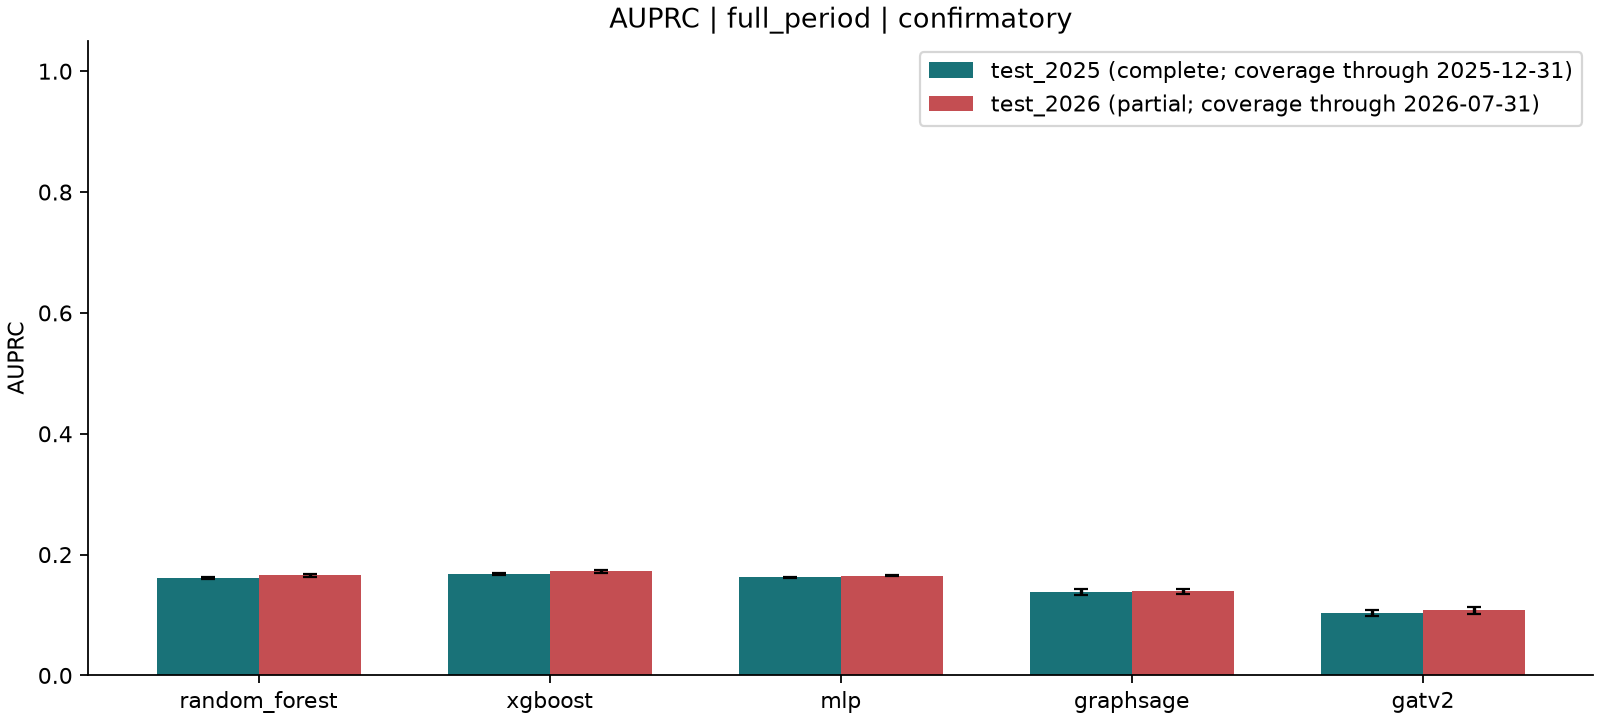
\includegraphics[width=\textwidth]{auprc-full_period.png}
\caption{AP dos modelos completos nos dois testes. O rótulo
\texttt{confirmatory} identifica o perfil técnico da execução, não
comprovação oficial da cobertura. O teste de 2026 é parcial.}
\label{fig:ap}
\end{figure}

\subsection{Comparação do custo computacional}

A Tabela~\ref{tab:custo-modelos} apresenta os custos dos modelos
completos, executados em CPU com uma \textit{thread} de modelo.
O tempo de treinamento corresponde ao ajuste do modelo, sem somar o
pré-processamento. Os tempos de inferência incluem a
verificação e o carregamento dos pesos e o pré-processamento do teste.
O RSS é o maior pico amostrado entre as cinco execuções, incluindo
processo, filhos, dados e bibliotecas; não mede apenas a memória
incremental do modelo.

% Fonte: resultados/computational-summary.csv
\begin{table}[!ht]
\centering
\caption{Custo dos cinco modelos avaliados (conjunto completo de
atributos). Treino: média $\pm$
desvio-padrão; inferência: média entre sementes. Tempos em segundos
e pico de RSS em MiB.}
\label{tab:custo-modelos}
\small
\setlength{\tabcolsep}{4pt}
\resizebox{\textwidth}{!}{%
\begin{tabular}{lcccc}
\toprule
\textbf{Algoritmo} & \textbf{Treino (s)} &
\textbf{Inferência 2025 (s)} & \textbf{Inferência 2026 (s)} &
\textbf{RSS (MiB)} \\
\midrule
Random Forest & $154{,}85 \pm 1{,}05$ & 5,60 & 3,09 & 5.874,49 \\
XGBoost & $75{,}20 \pm 20{,}82$ & 2,58 & 1,53 & 6.001,33 \\
MLP & $271{,}99 \pm 148{,}44$ & 5,53 & 0,67 & 6.139,52 \\
GraphSAGE & $117{,}96 \pm 45{,}98$ & 6,40 & 84,90 & 6.303,03 \\
GATv2 & $450{,}83 \pm 27{,}63$ & 10,96 & 6,65 & 6.059,39 \\
\bottomrule
\end{tabular}%
}
\end{table}

XGBoost combinou a maior AP com o menor tempo médio de treinamento
entre os cinco modelos completos. MLP teve a menor média de
inferência em 2026; XGBoost, em 2025. Random Forest apresentou RSS
menor e manteve vantagem em precisão nos dois testes e F1 em 2025.
GATv2 teve o maior tempo médio de ajuste neste orçamento.

Os tempos foram medidos em ambiente compartilhado, sujeito a carga
concorrente e efeitos de cache. As diferenças de memória e tempo entre
as famílias não constituem uma avaliação isolada de
complexidade dos algoritmos.

\subsection{Síntese, limitações e reprodutibilidade}

XGBoost apresentou maior AP e AUROC médias nos dois testes temporais.
Random Forest ofereceu maior precisão nos dois testes e maior F1 em
2025; MLP teve a maior revocação. GraphSAGE e GATv2 não superaram as
referências tabulares em AP. Portanto, neste protocolo e orçamento,
não foi observado ganho das GNNs frente às referências, sem
estabelecer inferioridade universal das arquiteturas em grafo.

A interpretação permanece limitada pela cobertura temporal assumida,
pela ausência de históricos com disponibilidade anterior comprovada,
pela malha estática de 2018, pelas lacunas de atributos viários e pelo
orçamento de um único candidato de configuração por algoritmo. Além
disso, os dois testes reutilizam a mesma geografia: não foi validada
generalização para outras regiões. Sem denominador de fluxo de
tráfego, os resultados tratam de ocorrência registrada por
segmento--semana, não de taxa de risco ajustada à exposição nem de
efeitos causais. O desempenho operacional também não foi validado.

As tabelas foram obtidas dos artefatos do relatório experimental
\texttt{confirmatory}: \texttt{metrics.csv}, \texttt{populations.csv}
e \texttt{computational-summary.csv}, incluindo os cinco modelos.
As ablações vieram de \texttt{ablations.csv}. Os arquivos foram
preservados em \texttt{resultados/}, sem substituir valores por
resultados de testes sintéticos.
O recibo de reprodução de 23 de setembro de 2026 confirmou a
reconstrução do conjunto de dados e a repetição das inferências com
os pesos arquivados dos modelos e variantes do experimento,
sem acesso à rede e sem novo treinamento, com diferença máxima de 0,0
ponto percentual nas métricas verificadas. Essa verificação ocorreu em
processo separado e arquivos temporários, mas no mesmo ambiente Python
e bibliotecas instalados; não representa
replicação independente em outro computador. A cópia organizada
preserva o pacote original, com seu código e inventário congelados,
em \texttt{reproducao/confirmatory.tar.gz}. Este documento atualizado
é posterior à execução e não foi inserido retroativamente no pacote.

\clearpage
\section{Planejamento original e conclusão}

A Tabela~\ref{tab:cronograma} registra o planejamento original de
16 semanas; não é uma medição das datas efetivas de cada atividade.
Os artefatos de setembro de 2026 registram dados preparados,
treinamentos, avaliação e reprodução concluídos. A conclusão permanece
condicionada à hipótese de cobertura temporal e aos limites
metodológicos descritos neste texto. Novas buscas de parâmetros ou
atributos exigem outro protocolo, declarando que os testes atuais já
foram observados.

\begin{table}[ht]
\centering
\caption{Cronograma de execução (16 semanas)}
\label{tab:cronograma}
\begin{tabular}{>{\raggedright\arraybackslash}p{5.4cm}cccc}
\toprule
\textbf{Atividade} & \textbf{M1} & \textbf{M2} & \textbf{M3} & \textbf{M4} \\
\midrule
Revisão bibliográfica & $\bullet$ & $\bullet$ & & \\
Aquisição e preparação dos dados da PRF & $\bullet$ & $\bullet$ & & \\
Construção da malha rodoviária como grafo & & $\bullet$ & $\bullet$ & \\
Implementação dos modelos de referência & & & $\bullet$ & \\
Implementação das GNNs & & & $\bullet$ & \\
Treinamento e ajuste dos modelos & & & $\bullet$ & $\bullet$ \\
Avaliação e análise dos resultados & & & & $\bullet$ \\
Redação e revisão do artigo & & & $\bullet$ & $\bullet$ \\
\bottomrule
\end{tabular}
\end{table}



% ============================================================
\begin{thebibliography}{99}

\bibitem{prf2026}
Polícia Rodoviária Federal.
\newblock Balanço da PRF mostra redução da letalidade nas BRs em 2025.
\newblock Governo Federal, fev. 2026.
\newblock Disponível em: \url{https://www.gov.br/prf/pt-br/noticias/nacionais/2026/fevereiro/menos-mortes-e-feridos-balanco-da-prf-mostra-reducao-da-letalidade-nas-brs-em-2025}

\bibitem{araujo2022}
R. B. de Araújo.
\newblock Regras de associação entre as características dos veículos e os
acidentes de trânsito em rodovias federais brasileiras por meio de
aprendizado de máquina.
\newblock Dissertação de Mestrado, UFMG, 2022.
\newblock Disponível em: \url{https://repositorio.ufmg.br/items/829406e3-546d-438c-88ce-d22fc18bba88}

\bibitem{zhang2026}
Z. Zhang, M. Duan, H. N. Koutsopoulos e H. R. Zhang.
\newblock Learning Multimodal Embeddings for Traffic Accident Prediction
and Causal Estimation.
\newblock In: \textit{Proc. KDD 2026}, Jeju Island, 2026.
\newblock Disponível em: \url{https://arxiv.org/abs/2512.02920}

\bibitem{nippani2023}
A. Nippani, D. Li, H. Ju, H. Koutsopoulos e H. Zhang.
\newblock Graph Neural Networks for Road Safety Modeling: Datasets and
Evaluations for Accident Analysis.
\newblock In: \textit{NeurIPS 2023 Datasets and Benchmarks}, 2023.
\newblock Disponível em: \url{https://arxiv.org/abs/2311.00164}

\bibitem{zhuang2024}
X. Gao, X. Jiang, D. Zhuang, H. Chen, S. Wang, S. Law e J. Haworth.
\newblock Uncertainty-Aware Probabilistic Graph Neural Networks for
Road-Level Traffic Accident Prediction.
\newblock \textit{arXiv:2309.05072v4}, 2024.
\newblock Disponível em: \url{https://arxiv.org/abs/2309.05072}

\bibitem{amorim2023}
B. de S. P. Amorim, A. A. Firmino, G. Braz Júnior et al.
\newblock A Machine Learning Approach for Classifying Road Accident
Hotspots.
\newblock \textit{ISPRS International Journal of Geo-Information}, v. 12,
n. 6, art. 227, 2023.
\newblock Disponível em: \url{https://www.mdpi.com/2220-9964/12/6/227}

\bibitem{hamilton2017}
W. L. Hamilton, R. Ying e J. Leskovec.
\newblock Inductive Representation Learning on Large Graphs.
\newblock In: \textit{NeurIPS}, 2017, p. 1024--1034.
\newblock Disponível em: \url{https://arxiv.org/abs/1706.02216}

\bibitem{brody2022}
S. Brody, U. Alon e E. Yahav.
\newblock How Attentive are Graph Attention Networks?
\newblock In: \textit{ICLR}, 2022.
\newblock Disponível em: \url{https://arxiv.org/abs/2105.14491}

\bibitem{chen2016}
T. Chen e C. Guestrin.
\newblock XGBoost: A Scalable Tree Boosting System.
\newblock In: \textit{Proc. KDD}, 2016, p. 785--794.
\newblock Disponível em: \url{https://arxiv.org/abs/1603.02754}

\bibitem{breiman2001}
L. Breiman.
\newblock Random Forests.
\newblock \textit{Machine Learning}, v. 45, n. 1, p. 5--32, 2001.
\newblock Disponível em: \url{https://doi.org/10.1023/A:1010933404324}

\bibitem{boeing2017}
G. Boeing.
\newblock OSMnx: New Methods for Acquiring, Constructing, Analyzing,
and Visualizing Complex Street Networks.
\newblock \textit{Computers, Environment and Urban Systems}, v. 65,
p. 126--139, 2017.
\newblock Disponível em: \url{https://doi.org/10.1016/j.compenvurbsys.2017.05.004}

\bibitem{who2023}
World Health Organization.
\newblock Global Status Report on Road Safety 2023.
\newblock WHO, Geneva, 2023.
\newblock Disponível em: \url{https://www.who.int/publications/i/item/9789240086517}

\end{thebibliography}

\end{document}
